\section{Additional model comparisons}
\label{app:task-09-10-extra}

These separate plots show the same results as the main performance and timing tables.

\begin{figure}[H]
\centering
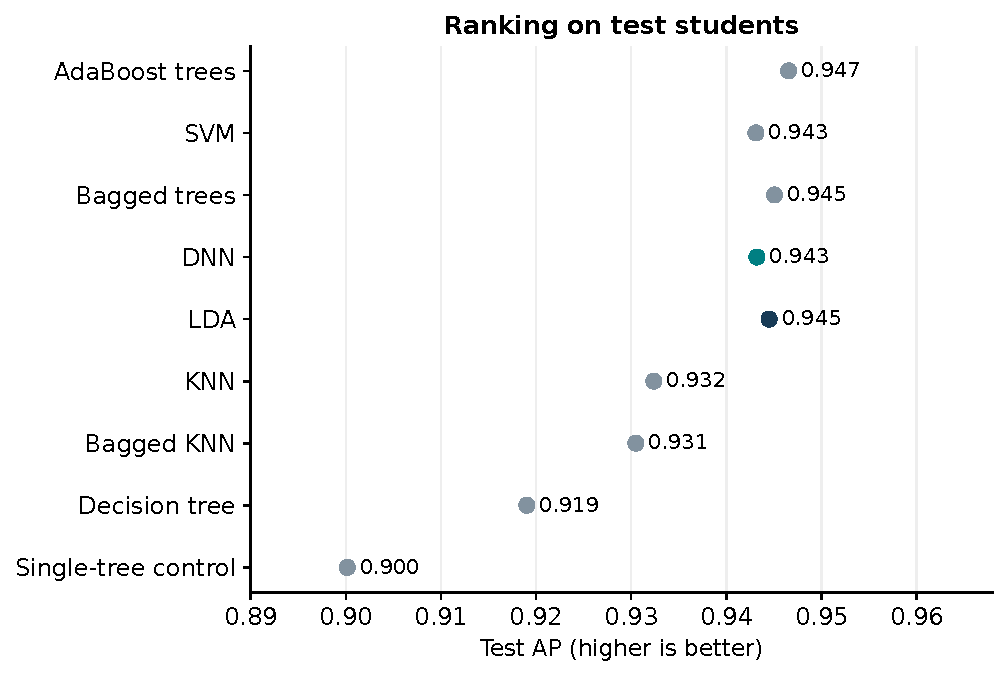
\includegraphics[width=0.74\linewidth]{Images/10_test_average_precision.pdf}
\caption[Held-out average precision]{AP on the same test students. Navy marks the recommended LDA classifier and teal the DNN. Rows follow the development ranking. Higher AP means better ranking of recorded dropout cases.}
\label{fig:test-ap}
\end{figure}

\begin{figure}[H]
\centering
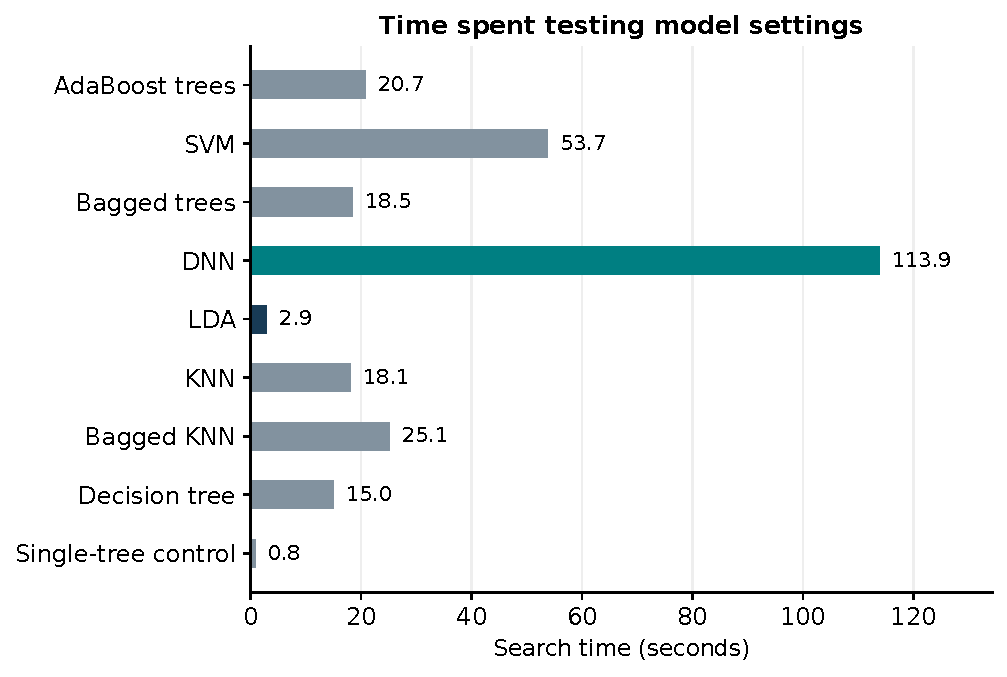
\includegraphics[width=0.74\linewidth]{Images/10_model_search_time.pdf}
\caption[Hyperparameter search time]{Time spent testing settings and fitting the selected model. Search budgets differ between algorithms.}
\label{fig:search-time}
\end{figure}

\begin{figure}[H]
\centering
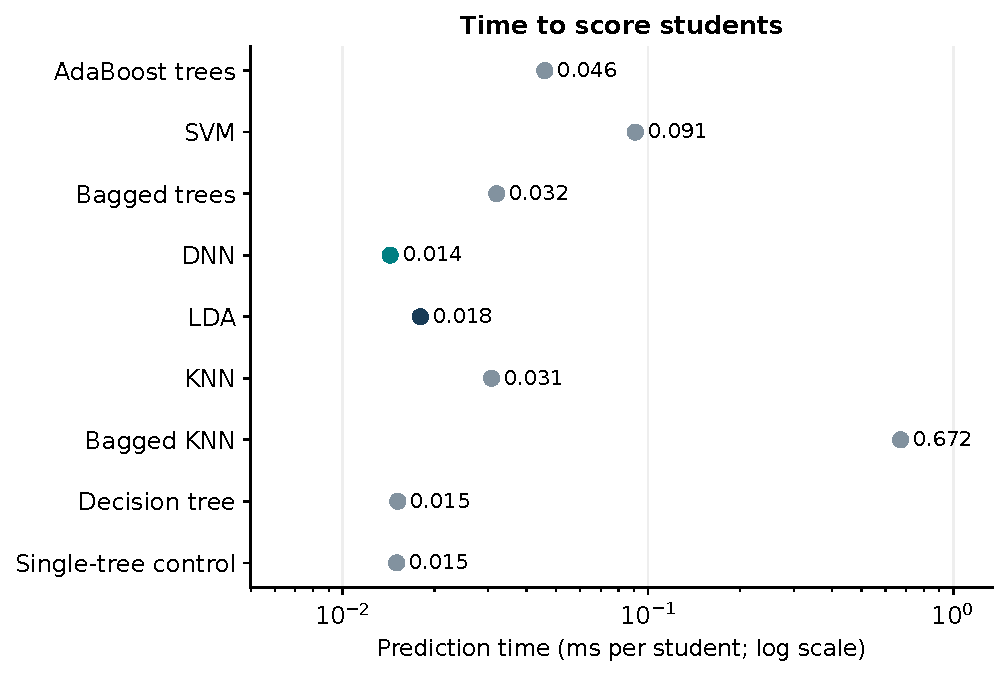
\includegraphics[width=0.74\linewidth]{Images/10_model_inference_time.pdf}
\caption[Batch prediction time per student]{Median of 25 prediction timings after three warm-up calls, including preprocessing, divided by the number of test students. The horizontal axis uses a logarithmic scale. The main timing table reports quartiles.}
\label{fig:inference-time}
\end{figure}
